\chapter{Software}
\label{chap:software}
%
% preface chapter
\lettrine[lines=3]{T}{his} chapter describes the software developed for the
hardware described in the chapter \ref{chap:hardware}. The choice to use the Qt
framework guarantees the portability and cross-platform support, as well
as the graphical interface and high data performance the feature of compiled
languages.  The software is divided into two programs capable of communicating
with each other: the first works on Raspberry Pi and allows the user to
interface easily with the FLIR thermal camera and with the Raspicam camera. 
It also acts as a TCP server to send the images shot to connected devices. 
The second part is a client program that receives the data sent by the main
device, and allows the analysis of the image through machine learning on
dedicated hardware.
%
% input files
%
\section{Signals \& Slots}
\label{ref:soft-signal-slot}
In the project extensive use was made of the Signal and Slot mechanism, this to
allow communication between the objects in the code. Signals and slots are used
for communication between objects. The signals and slots mechanism is a central
feature of Qt and probably the part that differs most from the features provided
by other frameworks. Signals and slots are made possible by Qt's meta-object
system.\cite{Qt:signal-slot}

\subsection{Introduction}
\label{ssec:soft-intro}
In GUI programming, when we change one widget, we often want another widget to
be notified. More generally, we want objects of any kind to be able to
communicate with one another.

Other toolkits achieve this kind of communication using callbacks. A callback is
a pointer to a function, so if you want a processing function to notify you
about some event you pass a pointer to another function (the callback) to the
processing function. The processing function then calls the callback when
appropriate. While successful frameworks using this method do exist, callbacks
can be unintuitive and may suffer from problems in ensuring the type-correctness
of callback arguments.\cite{Qt:signal-slot}

\subsection{Signals and Slots}
\label{ssec:soft-sig-solt-detail}
In Qt, we have an alternative to the callback technique: We use signals and
slots. A signal is emitted when a particular event occurs. Qt's widgets have
many predefined signals, but we can always subclass widgets to add our own
signals to them. A slot is a function that is called in response to a particular
signal. Qt's widgets have many pre-defined slots, but it is common practice to
subclass widgets and add your own slots so that you can handle the signals that
you are interested in. 
%
%
\begin{figure}[htb]
	\centering
	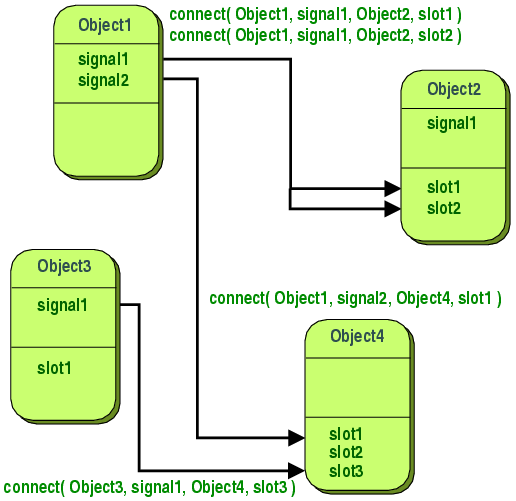
\includegraphics[width=0.65\textwidth]{abstract-connections.png}
	\caption{Signal and Slot scheme.}
	\label{fig:software-signal-slots-scheme}
\end{figure}
%
The signals and slots mechanism is type safe: The signature of a signal must
match the signature of the receiving slot. (In fact a slot may have a shorter
signature than the signal it receives because it can ignore extra arguments.)
Since the signatures are compatible, the compiler can help us detect type
mismatches when using the function pointer-based syntax. The string-based SIGNAL
and SLOT syntax will detect type mismatches at runtime. Signals and slots are
loosely coupled: A class which emits a signal neither knows nor cares which
slots receive the signal. Qt's signals and slots mechanism ensures that if you
connect a signal to a slot, the slot will be called with the signal's parameters
at the right time. Signals and slots can take any number of arguments of any
type. They are completely type safe.

All classes that inherit from QObject or one of its subclasses (e.g., QWidget)
can contain signals and slots. Signals are emitted by objects when they change
their state in a way that may be interesting to other objects. This is all the
object does to communicate. It does not know or care whether anything is
receiving the signals it emits. This is true information encapsulation, and
ensures that the object can be used as a software component.

Slots can be used for receiving signals, but they are also normal member
functions. Just as an object does not know if anything receives its signals, a
slot does not know if it has any signals connected to it. This ensures that
truly independent components can be created with Qt.

You can connect as many signals as you want to a single slot, and a signal can
be connected to as many slots as you need. It is even possible to connect a
signal directly to another signal. (This will emit the second signal immediately
whenever the first is emitted.)

Together, signals and slots make up a powerful component programming mechanism.\cite{Qt:signal-slot}

\subsection{Signals}
\label{ssec:soft-signal}
Signals are emitted by an object when its internal state has changed in some way
that might be interesting to the object's client or owner. Signals are public
access functions and can be emitted from anywhere, but we recommend to only emit
them from the class that defines the signal and its subclasses.

When a signal is emitted, the slots connected to it are usually executed
immediately, just like a normal function call. When this happens, the signals
and slots mechanism is totally independent of any GUI event loop. Execution of
the code following the emit statement will occur once all slots have returned.
The situation is slightly different when using queued connections; in such a
case, the code following the \textbf{\texttt{emit}} keyword will continue
immediately, and the slots will be executed later.

If several slots are connected to one signal, the slots will be executed one
after the other, in the order they have been connected, when the signal is
emitted.

Signals are automatically generated by the \emph{moc} and must not be implemented in
the \texttt{.cpp} file. They can never have return types (i.e. use void).\cite{Qt:signal-slot}

\subsection{Slots}
\label{ssec:soft-slots}
A slot is called when a signal connected to it is emitted. Slots are normal C++
functions and can be called normally; their only special feature is that signals
can be connected to them.

Since slots are normal member functions, they follow the normal C++ rules when
called directly. However, as slots, they can be invoked by any component,
regardless of its access level, via a signal-slot connection. This means that a
signal emitted from an instance of an arbitrary class can cause a private slot
to be invoked in an instance of an unrelated class.

Compared to callbacks, signals and slots are slightly slower because of the
increased flexibility they provide, although the difference for real
applications is insignificant. In general, emitting a signal that is connected
to some slots, is approximately ten times slower than calling the receivers
directly, with non-virtual function calls. This is the overhead required to
locate the connection object, to safely iterate over all connections (i.e.
checking that subsequent receivers have not been destroyed during the emission),
and to marshall any parameters in a generic fashion. While ten non-virtual
function calls may sound like a lot, it's much less overhead than any
\texttt{new} or \texttt{delete} operation, for example. As soon as you perform a
string, vector or list operation that behind the scene requires \texttt{new} or
\texttt{delete}, the signals and slots overhead is only responsible for a very
small proportion of the complete function call costs. The same is true whenever
you do a system call in a slot; or indirectly call more than ten functions. The
simplicity and flexibility of the signals and slots mechanism is well worth the
overhead, which your users won't even notice.\cite{Qt:signal-slot}

%
% introduction
\section{Interface}
\label{sec:raspberry-software}
As anticipated, the software run on the Raspberry Pi is made following the
paradigm of object-oriented programming. Made in C++/Qt making extensive use
of the proprietary classes of the framework and the Standard Template Library
(STL). This program has some dependencies with regard to the thermal camera
drivers supplied by the manufacturer and are 32-bit, since the Raspberry Pi 3,
described in \ref{sec:raspi3}, is equipped with a 32-bit ARM Cortex-A53
processor. These allow total control of the camera. The second dependency is the
Raspicam library which allows the interface with the RGB camera allowing the
image acquisition.
%
\begin{figure}[htb]
	\centering
	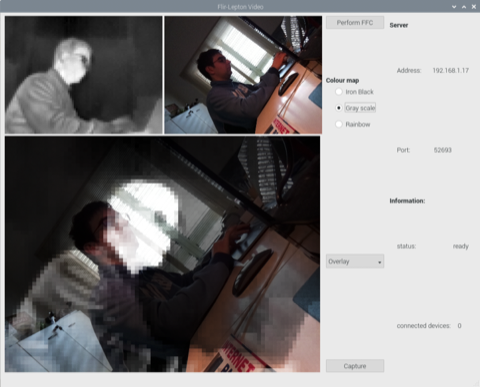
\includegraphics[width=0.65\textwidth]{grayscale.png}
	\caption{User interface run on Raspberry Pi 3b.}
	\label{fig:software-main-ui}
\end{figure}
%
% interface
Continuing a user interface has been created through the use of widgets, this is
divided into three areas. The first area shows the video streams acquired
separately in two labels, the third larger label shows the two streams mixed
through filters made available as default the overlay filter is used. It was
preferred not to perform a match of the images with pixel-by-pixel recalculation
for two reasons: the first due to the high difference in size of the sensors as
that of the thermal camera is $80 \times 60$ pixels while the Raspicam is $3280
\times 2464$ pixels. Furthermore motivation is due to not aggravate the 
computational load on the CPU.
The second area provides some controls for the user, in fact it is
possible to save thermal images on files during the acquisition. you can change
the heat map applied to the image on the fly by choosing from three different
possibilities, in the figure you can observe the result. 
Finally, it is possible to modify the mixing filter, also on the fly, of the
video streams to obtain different effects to improve visibility or to increase
details.
The last section of the user interface shows the information relating
to the TCP socket used for sending the video stream to other devices.
%
% image ui
\begin{figure}[htb]
    \centering
    \subfloat[][\emph{lava}.\label{subfig:lava-map}]
        {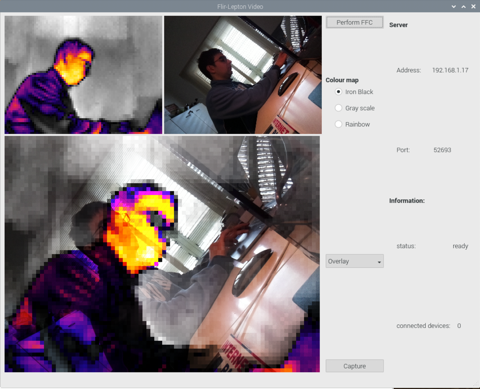
\includegraphics[width=.30\textwidth]{lava.png}} \quad
    \subfloat[][\emph{grayscale}.\label{subfig:grayscale-map}]
        {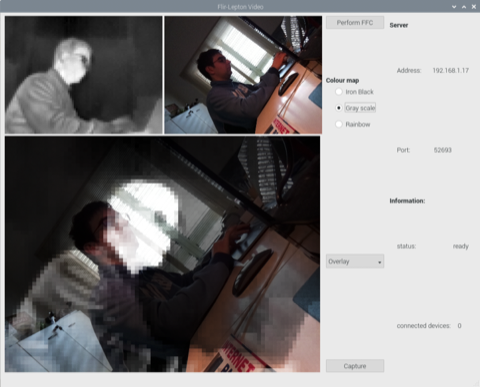
\includegraphics[width=.30\textwidth]{grayscale.png}} \quad
    \subfloat[][\emph{rainbow}.\label{subfig:rainbow-map}]
        {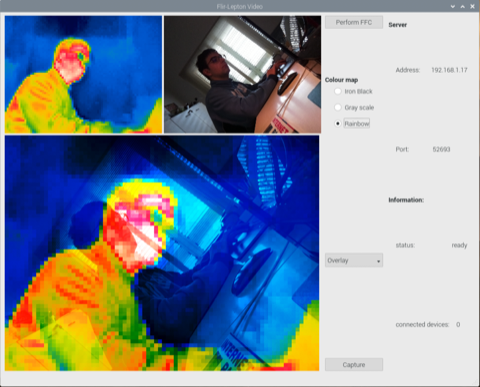
\includegraphics[width=.30\textwidth]{rainbow.png}}
    \caption{Result colourization applied to thermal camera data.}
    \label{fig:reuslt-maps}
\end{figure}
%
% software analysis 
\subsection{Software Analysis}
\label{ssec:raspberry-softw-analysis}
The user interface is run on the main thread, in order to maximize the
performance of the executed code the image acquisition operation is performed in
the secondary thread. Thanks to the use of the signal and slot system of Qt, 
introduced before in (\ref{ref:soft-signal-slot}), it is possible to update the 
labels without blocks typical of multi-threaded programming. 
The difficulty of concurrent programming usually consists in
synchronizing the access to resources by different threads that act in
competition on the same resources. Having two or more threads accessing the same
data simultaneously can lead to unexpected and unwanted results. 
In fact, without the application of particular programming techniques, it is not
possible to predict in a deterministic way, at the time of execution, when that
specific thread will be executed: their progression depends on the priorities
decided by the scheduler of the operating system and not by the programmer. 
In fact, multiple threads can access the same variable and modify its content or
value. Therefore, synchronization techniques such as mutual exclusion are used
to solve the problem. As a result, ideally a thread should execute code as
independent of the rest of the program as possible. Furthermore, errors in
synchronization between threads are often very difficult to detect because their
occurrence essentially depends on the environment in which the program is run.
The synchronization of one thread with another is normally necessary to allow
them to communicate with each other and to return the results of a function to
the main process; it is normally done through \emph{mutex}\cite{wiki:thread}.
Analysing the code of the thread that takes care of acquiring the images we can 
see that it proceeds without mutex\footnote{The mutex class is a synchronization
primitive that can be used to protect shared data from being simultaneously
accessed by multiple threads.}, but uses the signal and slot system as mentioned
before.
%
% code list
\inputminted[frame=lines,framesep=2mm, linenos=true, autogobble, breaklines=true, fontsize=\scriptsize, firstline=36, lastline=100]{c++}{software/code/leptonthread.cpp} 
\captionof{listing}{Infinite loop thread cameras.\label{lst:rasp-leptonthread}}
%
\pagebreak
Going to analyse in detail the infinite loop, reported in the
listing (\ref{lst:rasp-leptonthread}), executed in a thread other than the main
one that manages only the main interface, it can be observed that:
\begin{itemize}
\item (line 37--56) When the function starts, an instance of the \texttt{QImage}
type object is instantiated to contain the image acquired during the cycle. The
parameters of the frame size are provided and the color space this allows to
increase the speed of the cycle as it will not be cyclically cancelled and
reallocated the same, but will be reused. The communication with the thermal
camera is opened via the SPI port if the cycle is not started or if the
communication is interrupted the communication is closed.
% code list
%\begin{minipage}{\linewidth}
%\centering
%\inputminted[bgcolor=bg,frame=lines,framesep=2mm, linenos=true, autogobble, breaklines=true, fontsize=\scriptsize, firstline=36, lastline=61]{c++}{software/code/leptonthread.cpp} 
%\captionof{listing}{Data acquisition from SPI.}
%\label{lst:rasp-leptonthread-data} 
%\end{minipage}
%
\item (line 66--78) The main cycle is to acquire data from the saved camera
registers, as the order is MSB\footnote{MSB can also stand for "most significant
byte". \emph{Big-endian processor}: When data is loaded into a multi-byte
register, the first byte (with the lowest address) is the most significant byte
of the data.\cite{56322}}, reversed in according to LSB\footnote{LSB can also
stand for "least significant byte". \emph{Little-endian processor}: When data is
loaded into a multi-byte register, the first byte (with the lowest address) is
the least significant byte of the data.\cite{56322}}. The values are then scaled
to obtain a consistent representation of the hot and cold areas. Then the color
map is applied to color the raw data obtained from the scaling process described
above.
%% code list
%\begin{minipage}{\linewidth}
%\centering 
%\inputminted[bgcolor=bg,frame=lines,framesep=2mm, linenos=true, autogobble, breaklines=true, fontsize=\scriptsize, firstline=79, lastline=108]{c++}{software/code/leptonthread.cpp} 
%\captionof{listing}{Flip the MSB and LSB and colouration.} 
%\label{lst:rasp-leptonthread-MSB-LSB} 
%\end{minipage}\linebreak
%%
\item (line 79--97) Finally, signals are output for the coloured thermal image,
for the RGB image acquired by the Raspicam library and passed through the slot
and the last resulting from mixing of previous two depend on effect of selected
in UI interface.
%% code list
%\begin{minipage}{\linewidth}
%\centering 
%\inputminted[bgcolor=bg,frame=lines,framesep=2mm, linenos=true, autogobble, breaklines=true, fontsize=\scriptsize, firstline=36, lastline=117]{c++}{software/code/leptonthread.cpp} 
%\captionof{listing}{Infinite loop thread cameras.} 
%\label{lst:rasp-leptonthread} 
%\end{minipage}
\end{itemize}
As can be seen, the cycle proceeds without mutuals or blocking conditions, in
fact, as previously described, it is possible to change the color map or the
mixing tool on the fly.
%
% analysing comunication
% description socket tcp
\newpage
\section{Communication systems}
\label{sec:software-TCPSocket}
In digital data communications, wiring together two or more devices is one of
the first steps in establishing a network. As well as this hardware requirement,
software must also be addressed. The Open System Interconnection (OSI) model
proposed by the International Organization for Standardization (ISO) is a
standard way to structure communication software that is applicable to any
network. The model has been standardized by ISO and International
Telecommunication Union (ITU) Telecommunication Standardization Sector (ITU-T)
which is the organization coordinating standards for telecommunications. 
The
communication is based on low-level message passing between the communicating
systems.
\begin{itemize}
\item A wants to communicate with B; 
\item A builds a message addressing B; 
\item A executes a call to the communication module to send the message to B.
\end{itemize}
Of course, A and B need to speak the same language, i.e., they need to agree on the meaning
of the bits being sent. The protocols define the rules for communication. 
When
data is exchanged through a computer network, the system rules are called a
network protocol. A protocol must define the syntax, semantics, and timing of
communication (i.e. how, what and when); the specified behaviour is typically
independent of how it is to be implemented. Syntax: refers to the structure or
the format of the data. Semantics: the way in which the bit patterns are
interpreted. Timing: specify when the data can be sent and how fast it will be.
Another term is synchronization.
The communication between two nodes of a network occurs by sending messages. a
message is broken down into a sequence of packets, and each packet is
transmitted individually.
The structure includes some control bits at the beginning of the message called
\emph{header} and at the end called \emph{footer}.
the control bits can contain information such as: the sending node of the
packet, the recipient node of the package, package length information,
information that allows you to verify the correctness of the package. \cite{mandrioli2008informatica}
%
% %TODO Insert image
% image 
%
\subsection{Architecture}
\label{ssec:soft-client-server}
Client/server architectures are based on the functional division of IT
applications into two categories. Few computers act as servers, run a particular
program that allows the computer to receive requests and send replies.
As shows in figure (\ref{fig:client-server architecture}).\hfill \break
The clients, on the other hand, run a program that allows them to send requests and
receive replies. Client/server applications are two-level architectures, that
is, the first level is the client and the second level is the server. The
interaction protocols between client and server are quite simple. among the
advantages of client/server architectures we have the simplicity of
construction and the possibility of having easy-to-use clients.\\ 
Disadvantages include the risk of overloading the computer acting as a server 
and the communication channel with which the server is connected to the network.\cite{mandrioli2008informatica}\hfill \break
%
%
\begin{figure}[ht]
	\centering
	\resizebox{0.65\textwidth}{!}{\begin{tikzpicture}[block/.style={draw,minimum width=2cm,minimum height=1cm}, font=\sffamily] 
\node[block](C) {Client}; 
\node[block,right=9cm of C](S) {Server}; 
\draw[-latex] (C.15) -- (S.165)	node[midway,above]{Request}; 
\draw[-latex] (S.195) -- (C.-15) node[midway,below]{Response}; 
\end{tikzpicture}}
	\caption{Two level client/server architecture} 
	\label{fig:client-server architecture}
\end{figure}
%
\newline In the Internet protocol suite there is also the Transmission Control Protocol
(TCP). It is the complement of the Internet Protocol, yielding the well known
TCP/IP. TCP provides reliable, ordered, and error-checked delivery of the
messages between applications on an IP network. The most used internet
applications, i.e. the World Wide Web, e-mail, file transfer, rely on TCP.
%
\subsection{Server implementation}
\label{ssec:soft-rasp-server}
In our case, it implements \texttt{QTcpSocket} network communication.  So, there
is a server service in main program shows in figure
(\ref{fig:software-socket-server}). While there is a client application deepened
later in section (\ref{sec:software-coral-intro}). Server application has
\texttt{QTcpSocket} and it listens to some port, in our case $52693$.
 Client has \texttt{QTcpSocket}, but has not connected to the server yet:\linebreak
%
%
\begin{figure}[!ht]
	\centering
	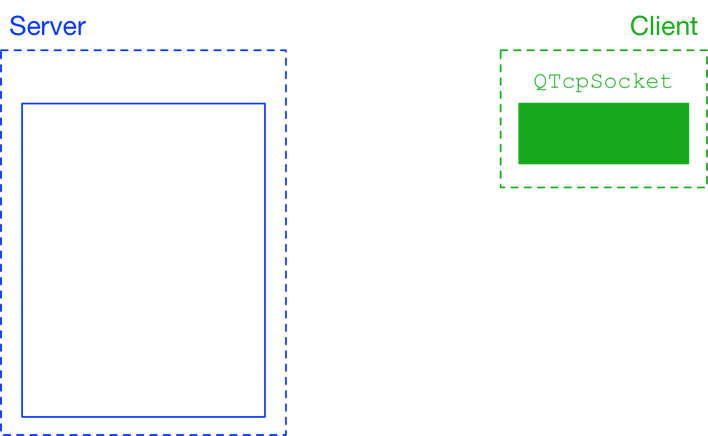
\includegraphics[width=0.7\textwidth]{qtcpserver-qtcpsocket.png}
	\caption{Interface client server \texttt{QTcpSocket}.}
	\label{fig:software-socket-server}
\end{figure}
%
\\When client connects to server, a \texttt{QTcpSocket} is created on the server’s
side, through which server and client can talk to each other and start send
message, shows in figure (\ref{fig:software-socket-server-client}).
%
%
\begin{figure}[htb]
	\centering
	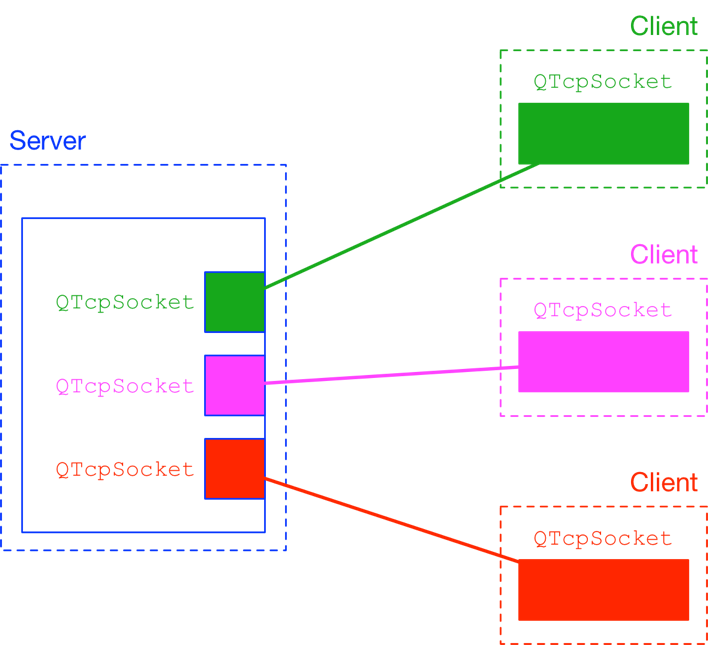
\includegraphics[width=0.55\textwidth]{qtcpserver-qtcpsocket-clients.png}
	\caption{Connection between server-clients.}
	\label{fig:software-socket-server-client}
\end{figure}
%
In particular, we observe the function reported in (\ref{lst:rasp-code-thread})
implemented in server application which sends the image just captured by the RGB
camera to the server to be  encapsulated in the message before send. 
In the function it is possible to observe the presence of a mutex which is 
locked to protect the resource and avoid overwriting through function calls.
The frame, i.e. the resource, is converted and stored in buffer before
sending.\\ 
Upon exiting the function body, the mutex is unlocked, thus giving free
access to resources again.
% code list
\begin{listing}[ht]
\inputminted[frame=lines,framesep=2mm, linenos=true, autogobble, breaklines=true, fontsize=\scriptsize, firstline=84, lastline=95]{c++}{software/code/mainwindow.cpp} 
\caption{Particular report function sending image.} 
\label{lst:rasp-code-thread} 
\end{listing}

%
% introduction
\section{Client}
\label{sec:software-coral-intro}
The software that acts as a client on the Coral dev-board, presented in chapter
\ref{}, created by Google is based on the same Qt framework previously
introduced in order to guarantee portability and reliability of the code. This,
remember, has an ARM Cortex-A53 processor, but unlike the one mounted on
Raspberry it executes 64-bit code and takes advantage of the new armv8
architecture with a significant performance gain. This difference arises from
the execution of Machine Learning operations supported by the TPU, described in
detail in section \ref{}.
%
% interface
As seen for the main program, here too we find a main interface executed in the
main thread. The simplest interface is divided into two areas: the first one
where it is possible to observe the flow of images coming from the TCP socket
analyzed later. The second, on the other hand, offers the possibility of
connecting to the TCP socket by entering the address and port of the machine on
which the server is run, which is listening for possible connection requests.
Once the connection between server and client is established, the label is
updated with the images received.
%
% software analysis
\subsection{Software Analysis}
\label{ssec:software-coral-analysis}
To avoid blockages and unpleasant delays in receiving images from the TCP
socket, multi-thread programming was used. In fact, as previously described, the
interface managed by QWidget is run on the main thread. If the connection is
stable, the thread starts which allows reception in a queue waiting to leave.\\ 
On the other hand, this is prepared when the class is instantiated within the
main function. Since this infinite cycle is the critical factor, we analyse its
structure in detail below.
%
% code list
\begin{listing}[ht] 
\inputminted[frame=lines,framesep=2mm, linenos=true, autogobble, breaklines=true, fontsize=\scriptsize, firstline=12, lastline=26]{c++}{software/code/streamerthread.cpp} 
\caption{Particular report function sending image.} 
\label{lst:coral-client-code} 
\end{listing}
%
\\As you can see in the function code, shown in Listing
(\ref{lst:coral-client-code}), we observe the instance of the \texttt{socket}
member object of the \texttt{QTcpSocket} class type. 
By starting the connection, the server. 
The critical section from the \emph{while loop} is protected by a mutex,
highlighted by the \texttt{QMutexLocker} class, a mutex indicates a
process of synchronization between concurrent processes or threads, with which
multiple parallel tasks are prevented from simultaneously accessing 
data in memory or other resources subject to race condition.\cite{wiki:mutex} 
Locking and unlocking a \texttt{QMutex} in complex functions and statements or
in exception handling code is error-prone.
\texttt{QMutexLocker} can be used in such situations to ensure that the state of the
mutex is always well-defined. \texttt{QMutexLocker} should be created within a
function where a \texttt{QMutex} needs to be locked. The mutex is locked when
\texttt{QMutexLocker} is created. If locked, the mutex will be unlocked when
the \texttt{QMutexLocker} is destroyed.
Using \texttt{QMutexLocker} greatly simplifies the code, and makes it more
readable.\cite{Qt:QMutexclass}
The buffer is filled with reading from the socket and before putting the signal
to update the image in the interface a small interval of time is waited to
guarantee the complete reception of the image.
Before updating the label on the dashboard, filter the image to verify that it
is consistent and different from an empty or corrupt image, shows in listing
(\ref{lst:coral-ui-code}). 
If this occurs, the function is immediately exited to
avoid viewing an image being ready to receive a new image. 
%
% code list
\begin{listing}[ht] 
\inputminted[frame=lines,framesep=2mm, linenos=true, autogobble, breaklines=true, fontsize=\scriptsize, firstline=88, lastline=100]{c++}{software/code/tcpclient.cpp} 
\caption{Implantation filter.} 
\label{lst:coral-ui-code} 
\end{listing}
%
% cnn part
\subsection{CNN-PART-TPU-INFERENCE}
%TODO
...

\section{Inference}
\label{sec:soft-inference}
%
%
In this section the inference process is analyzed on the neural network model,
taking into account that the two applications share the same code. In fact, when
the model is loaded into the buffer, it is interpreted by the TensorFlow Lite
library, returning the training information of the model and in particular the
information regarding the input and output of the model.
For this case, where you are interested in the problem of object detection, the
size of the image is requested at the input and the number of color channels in
this case is constant and fixed at three.
Furthermore, the function reported in listing (\ref{lst:inference-support}) is
analyzed, which allows you to adapt the model input with the data, that is, the
images coming from the camera, taking into account the nedd to satisfy the
neural model input and to adapt the information for the tensor calculation if in
floating point, or in 8-bit integers.
It also takes into account the process of quantization that took place during
the transformation from original model to lite model, in fact the input will
also be recalculated.
%
%
\begin{listing}[!h] 
\inputminted[frame=lines,framesep=2mm, linenos=true, autogobble, breaklines=true, fontsize=\scriptsize, firstline=29, lastline=70]{c++}{software/code/model_support_function.hpp} 
\caption{function that adapts the input image to the input required by the neural model.} 
\label{lst:inference-support} 
\end{listing}
%
%
For fully integer models, the inputs are unsigned integer 8-bit.\\ 
The mean and standard deviation (\texttt{std\_dev}), calculated as in
\eqref{eq:stddev}, values specify how to \texttt{uint8} values map to the float
input values used while training the model.\\
The mean is the integer value from $0$ to $255$ that maps to floating point
\texttt{$0.0\text{f}$}. 
\begin{equation}
\label{eq:stddev}
\text{\texttt{std\_dev}} = \frac{255}{\text{\texttt{float}}_\text{max}-\text{\texttt{float}}_\text{min}}
\end{equation}
Different hardware may have preferences and restrictions that may cause slight
deviations when implementing the specification that result in implementations
that are not bit-exact. Whereas that may be acceptable in most cases, the nature
of machine learning (and deep learning in the most common case) makes it
impossible to provide any hard guarantees.\cite{tflite-8bit}\\
8-bit quantization approximates floating point values using the following
formula \eqref{eq:8-bit}.
\begin{equation}
\label{eq:8-bit}
\text{\texttt{real}}_\text{\texttt{value}} = ({\text{\texttt{int8}}_\text{value}-\text{\texttt{zero}}_\text{point}}) \times \text{\texttt{scale}} 
\end{equation}
%
Per-axis (aka per-channel in Conv ops) or per-tensor weights are represented by
\texttt{int8} two’s complement values in the range $[-127, 127]$ with zero-point equal to $0$. Per-tensor activations/inputs are represented by \texttt{int8} two’s
complement values in the range $[-128, 127]$, with a zero-point in range $[-128,
127]$.
%
%
\subsection{Architecture x86\_64}
\label{ssec:x86-bench-inference}
We analyze in particular the inference cycle following the reception of the
frame by the TCP socket described previously in section
(\ref{ssec:software-coral-analysis}). 
In figure (\ref{subfig:all-bench}) the captured process shows the functions
performed:
%
\begin{itemize}
	\item The dark green rectangle represents the socket's reception function.
	\item The lighter green rectangle, on the other hand, is the time needed to calculate the inference.
	\item The pink rectangle represents the time to update the image in the user interface.
\end{itemize}
%
Although only one thread is shown here, in the solution adopted the TensorFLow
Lite module uses 8 cores, but it is possible to set a number of cores greater
than or equal to 1.
Comparing the two figures (\ref{subfig:time-cycle}) and
(\ref{subfig:time-inference}) it is observed that the duration of the cycle is
approximately $64.376 \,\si{\milli\second}$ and the other hand the infercence time
is $54.251 \,\si{\milli\second}$.
This time includes the execution of the functions described above, from this it
is possible to deduce that the most onerous task in terms of time and the
reconstruction of the image by the socket inside the
\textbf{TcpClient::imageAvailable} function. 
Meanwhile, \textbf{ModelTesnorFLowLite::run}'s function starts after about $10
\,\si{\milli\second}$ to end almost simultaneously with the function. Then the
cycle repeats itself.
Performing the inference with the TensorFlow Lite model, described in section
(\ref{sec:soft-inference}), on a laptop equipped with an Intel i7-7820HQ CPU
$2.90 \,\si{\giga\hertz}$ processor shows the benefits due to compression and
quantization of the neural model.
In particular, it is observed that the average time is $78 \,\si{\milli\second}$
therefore a considerable performance boost if compared with the time required,
when using the uncompressed model, is considerably slower when compared to the
result obtained in this case.
Although it is important to note that if the required time drops on the one
hand, the number of false positive cases increases on the other. 
%
\begin{figure}[htb]
	\centering
	\subfloat[][\emph{thread}.\label{subfig:all-bench}]%
		{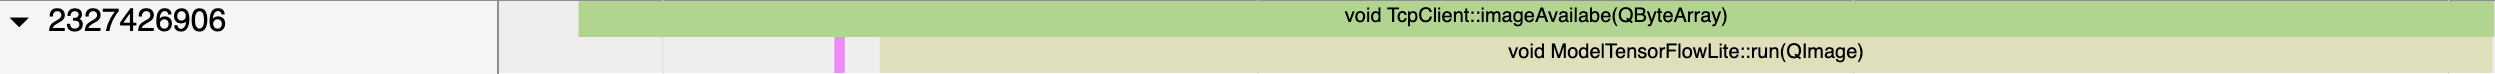
\includegraphics[width=\textwidth]{x86_64_1.jpg}} \\
	\subfloat[][\emph{time inference}.\label{subfig:time-inference}]%
		{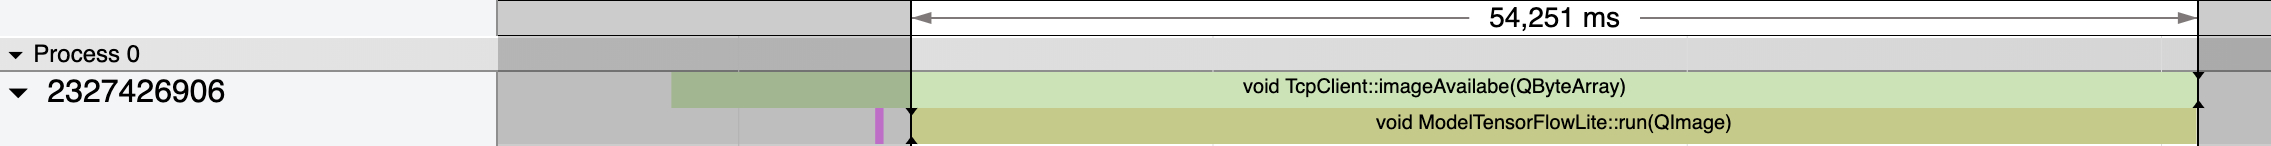
\includegraphics[width=\textwidth]{x86_64_2.jpg}} \\
	\subfloat[][\emph{total time cycle}.\label{subfig:time-cycle}]%
		{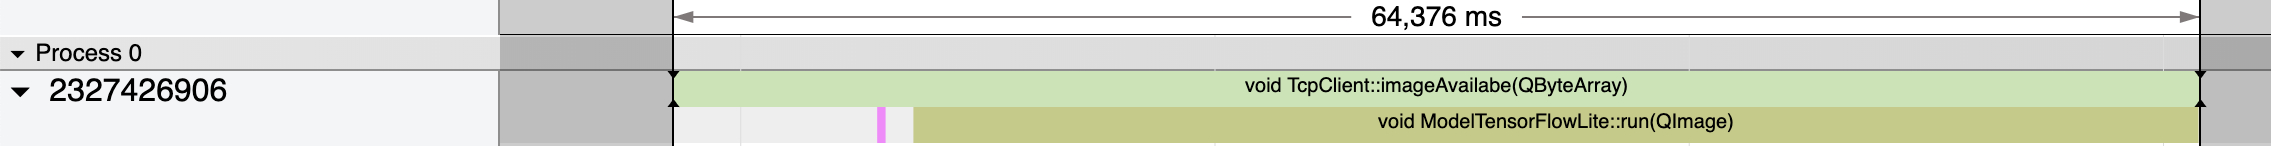
\includegraphics[width=\textwidth]{x86_64_3.jpg}}
	\caption{Visual benchmark inference on \texttt{x86\_64} architecture.}
	\label{fig:x86-bench}
\end{figure}
%
%
\subsection{Architecture armv7l}
\label{ssec:armv7l-bench-inference}
%
We now analyze the result of the execution of the inference process on the
hardware of the Raspberry Pi 3b computer board which mounts an ARM cortex-A53
processor.
In fact, the figures (\ref{fig:armv7l-bench}) show that the processes present a
different number and row, this is because parallel architecture is exploited and
in particular in the benchmark it has been possible to capture the distribution
of the tasks on the threads.
Unlike what is seen in the previous section, the inference is made immediately without
considering the expectation of the streaming of images by the socket.
The work cycle examined has a total duration of $694.296 \,\si{\milli\second}$,
please note that here too more than one core is assigned to the inference
process.
Moving forward in the analysis, we can distinguish within the cycle:
\begin{itemize}
	\item In green the image acquisition by the camera in the second thread.
	\item The orange rectangle the updating of the interface with the new image in the first thread.
	\item In bright green the execution of the function in the first thread that passes the image acquired by the camera to the function that performs the inference.
	\item The segment filled in olive green rectangle the inference process performed in the second thread.
\end{itemize}
As can be seen in figure (\ref{subfig:arm7-time-inference}), the inference process by the
\textbf{ModelTesnorFLowLite::run} function has an execution time of $528.105 
\,\si{\milli\second}$, considerably slower than the \texttt{x86\_64}
architecture previously discussed. although it has a longer execution time, the
whole program is not affected by this aspect due to the optimization carried out
by the compiler and by exploiting the multi-threading architecture as well as the
possibility of using SIMD\footnote{Single Instruction Multiple Data}
instructions.\\
Finally, we want to remember that both data come from the same code executed by
the machine, but two different architectures are being compared. 
The first encountered \texttt{x86\_64} supports 64-bit instructions, benefiting
from the larger size of the registers and in greater numbers, despite a much
higher clock frequency and being able to count on 4 physical and 4 virtual
cores. 
On the other hand the ARM process with \texttt{armv7l} architecture executes 32
bit instructions and has a much lower clock frequency.
%
\begin{figure}[htb]
	\centering
	\subfloat[][\emph{thread}.\label{subfig:arm7-all-bench}]%
		{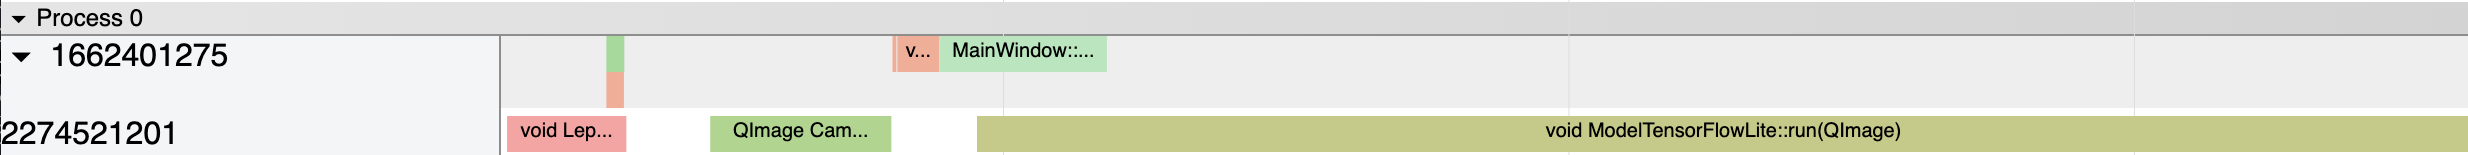
\includegraphics[width=\textwidth]{arm_32_1.jpg}} \\
	\subfloat[][\emph{time inference}.\label{subfig:arm7-time-inference}]%
		{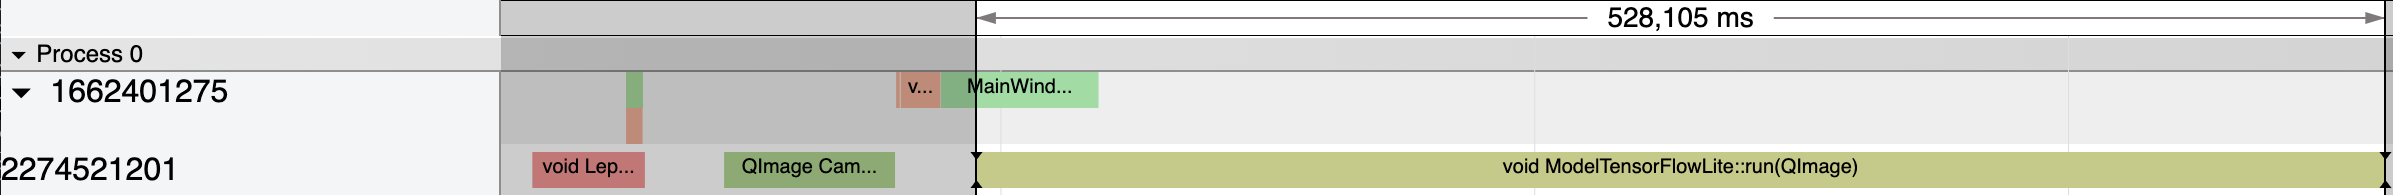
\includegraphics[width=\textwidth]{arm_32_2.jpg}} \\
	\subfloat[][\emph{total time cycle}.\label{subfig:arm7-time-cycle}]%
		{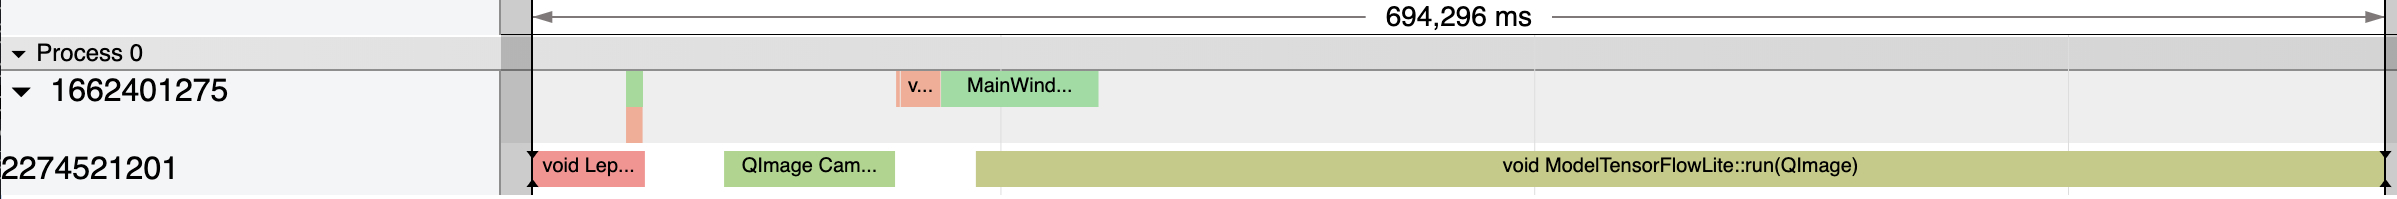
\includegraphics[width=\textwidth]{arm_32_3.jpg}}
	\caption{Visual benchmark inference on \texttt{armv7l} architecture.}
	\label{fig:armv7l-bench}
\end{figure}
%
\subsection{Architecture armv8a and TPU}
\label{ssec:tpu}
%
%
The last comparison is made on the processing capacity of Google's Coral
Dev-Board and in particular by the TPU that makes available for the tensor
calculation.
In the visual benchmark created in figure (\ref{subfig:TPU-all-bench}), unlike 
the previous ones, there is a single thread.
In this case it was not possible to isolate only the functions of interest, but 
all the calls to the functions made by the program were extracted.
In this analysis, unlike the previous ones, you are not using all the threads of
the processor that you remember is a 64-bit ARM cortex-A53.\\ 
The calculation is moved to the TPU thus relieving the main processor from the
calculation of the inference on the quantized model and compiled specifically to
operate on the unit.
Improvement can be observed with respect to the case of the execution of the
inference on the \texttt{armv7l} architecture in that when the times drop
drastically, in fact they are equal or better than to those seen in section
(\ref{ssec:x86-bench-inference}).\\  
The TPU processing unit performs the inference in approximately $36.317
\,\si{\milli\second}$ highlighted by the pink segment reported in figure 
(\ref{subfig:TPU-time-inference}) so called the \textbf{RunInference} 
function.
%
%
\begin{figure}[htb]
	\centering
	\subfloat[][\emph{thread}.\label{subfig:TPU-all-bench}]%
		{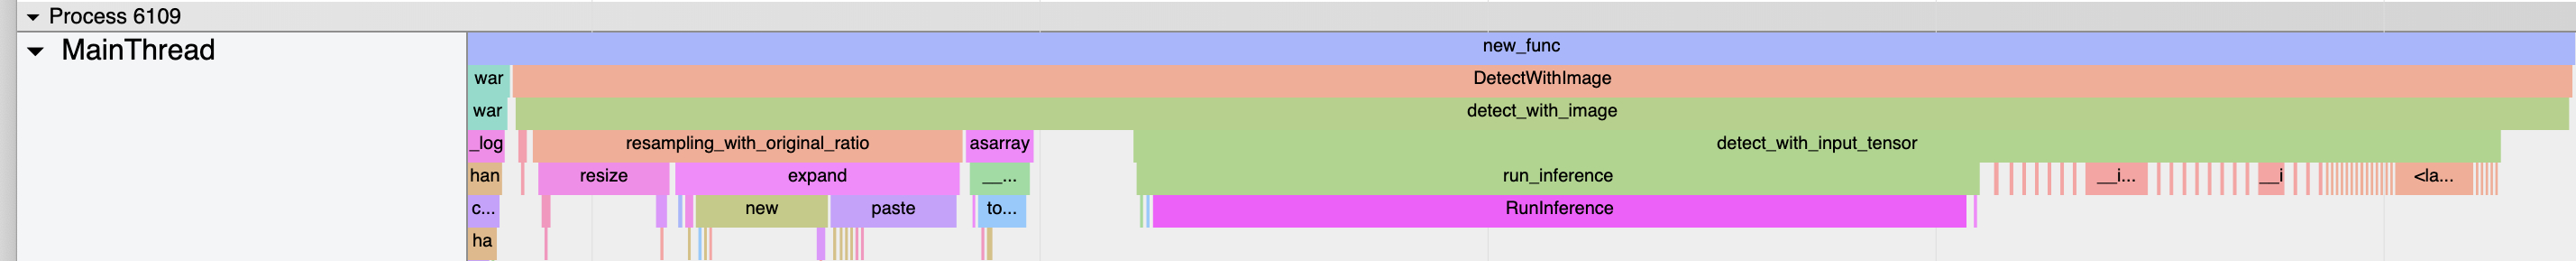
\includegraphics[width=\textwidth]{TPU_1.jpg}} \\
	\subfloat[][\emph{time inference}.\label{subfig:TPU-time-inference}]%
		{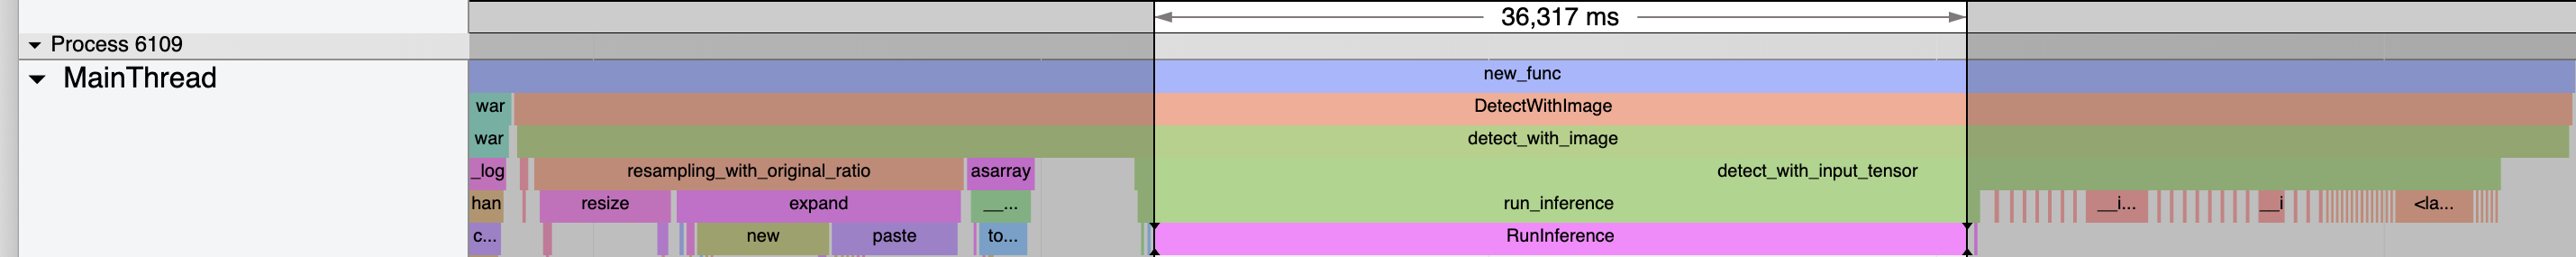
\includegraphics[width=\textwidth]{TPU_2.jpg}} \\
	\subfloat[][\emph{total time cycle}.\label{subfig:TPU-time-cycle}]%
		{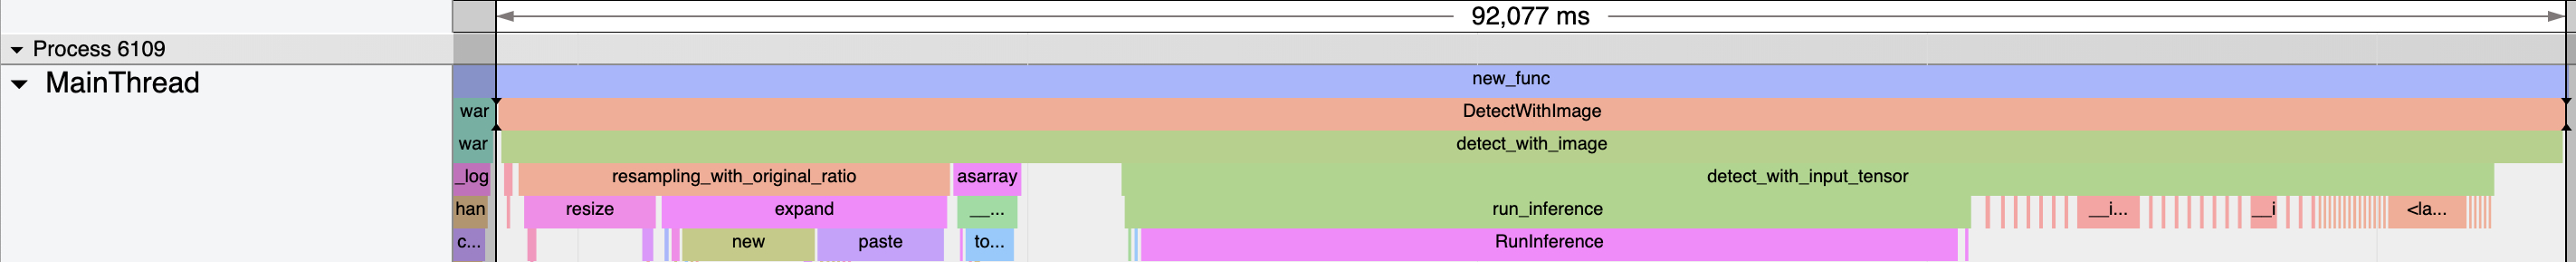
\includegraphics[width=\textwidth]{TPU_3.jpg}}
	\caption{Visual benchmark inference on \texttt{TPU}.}
	\label{fig:TPU-bench}
\end{figure}

As seen in (\ref{sec:hard-tpu}), the advantage of using TPU to perform largely derives
from the adoption of 8-bit integers that make tensor calculation easier.\\
Furthermore, the structure of the systolic array also guarantees benefits due to
the possibility of keeping the calculation time constant as the tensor
increases.
The entire inference calculation cycle is $92.077 \, \si{\milli\second}$ in
which the image arrives. The image is scaled to the desired input of the tensor
and ready to be analyzed, as observable in figure (\ref{subfig:TPU-time-cycle}).
